%%%%%%%%%%%%%%%%%%%%%%%%%%%%%%%%%%%%%%%%%%%%%%%%%%%%%%%%%%%%%%%%%%%%%%%%%
% $Id$
% %%%%%%%%%%%%%%%%%%%%%%%%%%%%%%%%%%%%%%%%%%%%%%%%%%%%%%%%%%%%%%%%%%%%%%%%%
%
% Transparencias para reunión de seguimiento HOFEM-AIRBUS sobre "Transmission
% /reflection" en HOFEM
%
% %%%%%%%%%%%%%%%%%%%%%%%%%%%%%%%%%%%%%%%%%%%%%%%%%%%%%%%%%%%%%%%%%%%%%%%%%
% Magia para que el acrobat reader lea bien el documento.
%\pdfobjcompresslevel=1

%\documentclass[notes,smaller,xcolor=table,dvipsnames]{beamer}
\documentclass[smaller,xcolor=table,dvipsnames]{beamer}

%\documentclass[notes,smaller,xcolor=table,dvipsnames,trans]{beamer}
%\documentclass[smaller,xcolor=table,dvipsnames,trans]{beamer}

%documentclass[notes,smaller,xcolor=table,dvipsnames,handout,hyperref={bookmarks=false}]{beamer}
%\documentclass[smaller,xcolor=table,dvipsnames,handout,hyperref={bookmarks=false}]{beamer}

%Ver uso de oprion onlyslideswithnotes  que no me parece funcionar


%\includeonlyframes{current}

\mode<handout>
{
  \usepackage{pgfpages}
%  \pgfpagesuselayout{2 on 1}[a4paper,border shrink=5mm]
%  \pgfpagesuselayout{4 on 1}[a4paper,landscape,border shrink=5mm]
  \nofiles
}

\usepackage{ifthen}
% \newboolean{ARCS} % Requiere package ``ifthen''
% \setboolean{ARCS}{FALSE} % Si true se personaliza algo para el curso
%                         % ARCS (antennas and RCS del MasteEADS)


% %%%%%%%%%%%%%%%%%%%%%%%%%%%%%%%%%%%%%%%%%%%%%%%%%%%%%%%%%%%%%%%%%%%%%%%%%

% $Id$

% %%%%%%%%%%%%%%%%%%%%%%%%%%%%%%%%%%%%%%%%%%%%%%%%%%%%%%%%%%%%%%%%%%%%%

% Estilo de los últimos años con linea azul al borde

% \mode<presentation>
% {
% %  \usetheme{Warsaw}
%   \usetheme{Boadilla}

%   \setbeamercovered{transparent}
%   % or whatever (possibly just delete it)

% \setbeamertemplate{navigation symbols}{}

% }

% \useoutertheme{uc3mcourse_updated2020} % curso de uc3m

% %%%%%%%%%%%%%%%%%%%%%%%%%%%%%%%%%%%%%%%%%%%%%%%%%%%%%%%%%%%%%%%%%%%%%

% Estilo de Sergio en traspas Radar, campos, etc

\usetheme{uc3m}


% %%%%%%%%%%%%%%%%%%%%%%%%%%%%%%%%%%%%%%%%%%%%%%%%%%%%%%%%%%%%%%%%%%%%%


%\setbeameroption{show notes on second screen=bottom}

%\setbeamersize{text margin right=0.1\linewidth,text margin left=0.1\linewidth}

\setbeamertemplate{frametitle continuation}[from second]

% \usepackage[spanish,es-noquoting,es-nolists,es-noshorthands]{babel}
%  \decimalpoint % utilizamos punto como separador decimal
%  \deactivatetilden % Desactiva abreviaciones ~n y ~N que dan muchos problemas.
% % %                Por ejemplo, con abreviaciones de bibtex como M.~N. Vouvakis
\usepackage[english]{babel}
% or whatever

% Tikz y derivados
%\input{preamble_tr_tikz}

%\usepackage[latin1]{inputenc}
\usepackage[utf8]{inputenc}
% or whatever

%\usepackage[T1]{fontenc}
% Or whatever. Note that the encoding and the font should match. If T1
% does not look nice, try deleting the line with the fontenc.
%\usepackage{times}
%\usepackage{lmodern}


\usepackage{amsmath}
\usepackage{amssymb}
%\usepackage{amscd} % conmutative diagrams
\usepackage{latexsym}

\usepackage{pifont}


\usepackage{verbatim}
\usepackage{listings}

  \lstdefinestyle{myFORTRANcode}
    {language=[90]Fortran,
    basicstyle=\ttfamily\footnotesize,
    keywordstyle=\color{blue}\ttfamily,
    stringstyle=\color{brown}\ttfamily,
    commentstyle=\color{red}\ttfamily,
    tabsize=2,
%    frame=single,
%    backgroundcolor=\color{yellow},
    breaklines=true,breakatwhitespace=true,prebreak=\space\&
  }
  \lstdefinestyle{myFORTRANcodeS} % S as "small"
    {language=[90]Fortran,
    basicstyle=\ttfamily\scriptsize,
    keywordstyle=\color{blue}\ttfamily,
    stringstyle=\color{brown}\ttfamily,
    commentstyle=\color{red}\ttfamily,
    tabsize=2,
%    frame=single,
%    backgroundcolor=\color{yellow},
    breaklines=true,breakatwhitespace=true,prebreak=\space\&
  }

  \lstdefinestyle{myFORTRANcodeOpenMP}
    {language=[90]Fortran,
    basicstyle=\ttfamily\footnotesize,
    keywordstyle=\color{blue}\ttfamily,
    stringstyle=\color{brown}\ttfamily,
    commentstyle=\color{red}\ttfamily,
    morecomment=[l]{\$},
    tabsize=2,
%    frame=single,
%    backgroundcolor=\color{yellow},
    breaklines=true,breakatwhitespace=false,prebreak=\space\&
  }


\usepackage{graphicx}
\usepackage{subfig}
%\usepackage{subfigure}


\usepackage{xmpmulti}

\usepackage{notacion}

% \usepackage{def_listas}

\usepackage{pdfpages}

\usepackage{multimedia}

\usepackage{array}  % Para tablas
\newcolumntype{C}{>{$}c<{$}} % Identificadores de columna en math mode
\newcolumntype{L}{>{$}l<{$}}
\newcolumntype{R}{>{$}r<{$}}

%\setlength{\arrayrulewidth}{0.5mm}
%\setlength{\tabcolsep}{18pt}
\setlength{\tabcolsep}{10pt}
\renewcommand{\arraystretch}{1.5}


\newcommand{\vbs}{\vspace{\baselineskip}}
\newcommand{\vbss}{\vspace{0.5\baselineskip}}
\newcommand{\vbsf}{\vspace*{\baselineskip}}
\newcommand{\vbssf}{\vspace*{0.5\baselineskip}}
\newcommand{\FIGURA}[1]{\vspace*{2\baselineskip} \centering{FIGURA \\ #1} \vspace*{2\baselineskip} }


\newcommand{\crule}{{\color{cyan} \hrule} }

\setcounter{tocdepth}{4}

% El paquete enumitem redefine las listas de Beamer:
%\usepackage{enumitem}
% \setitemize{label=\usebeamerfont*{itemize item}%
%    \usebeamercolor[fg]{itemize item}
%    \usebeamertemplate{itemize item}}

% Alternativa:
\newcounter{saveenumi}
\newcommand{\seti}{\setcounter{saveenumi}{\value{enumi}}}
\newcommand{\conti}{\setcounter{enumi}{\value{saveenumi}}}
\resetcounteronoverlays{saveenumi}





% %%%%%%%%%%%%%%%%%%%%%%%%%%%%%%%%%%%%%%%%%%%%%%%%%%%%%%%%%%%%%%%%%%%%%%%%%
%  Líneas para hacer versión con "notes" comentando cada traspa
%  Comentar las líneas para versión sin notes

% \usepackage{pgfpages}

% \setbeamertemplate{note page}[plain]
% \setbeameroption{show notes on second screen=bottom}
% \makeatletter
% \def\beamer@setupnote{%
%   \gdef\beamer@notesactions{%
%     \beamer@outsideframenote{%
%       \beamer@atbeginnote%
%       \beamer@notes%
%       \ifx\beamer@noteitems\@empty\else
%       \begin{itemize}\itemsep=0pt\parskip=0pt%
%         \beamer@noteitems%
%       \end{itemize}%
%       \fi%
%       \beamer@atendnote%
%     }%
%     \gdef\beamer@notesactions{}%
%   }
% }
% \makeatother

% %%%%%%%%%%%%%%%%%%%%%%%%%%%%%%%%%%%%%%%%%%%%%%%%%%%%%%%%%%%%%%%%%%%%%%%%%

% %%%%%%%%%%%%%%%%%%%%%%%%%%%%%%%%%%%%%%%%%%%%%%%%%%%%%%%%%%%%%%%%%%%%%%%%%

% Controla si se genera una version para alumno
% o no. En la version para alumno se omiten algunos detalles
\newboolean{alumno} % Requiere package ``ifthen''
%\setboolean{alumno}{TRUE}
\setboolean{alumno}{FALSE}

% %%%%%%%%%%%%%%%%%%%%%%%%%%%%%%%%%%%%%%%%%%%%%%%%%%%%%%%%%%%%%%%%%%%%%%%%%

\newcommand{\dirinputtex}{./inputtex}

\graphicspath{{./figures/}}
% \lstset{inputpath=./code_output}

\usepackage[nofancy]{rcsinfo}
\rcsInfo $Id: MTAC_MasterDays_2020.tex,v 1.1 2020/05/12 05:54:23 luise Exp luise $

% %%%%%%%%%%%%%%%%%%%%%%%%%%%%%%%%%%%%%%%%%%%%%%%%%%%%%%%%%%%%%%%%%%%%%%%%%


\title[HOFEM-AIRBUS(v{\rcsInfoRevision})]{HOFEM-AIRBUS Transmission/Reflection}

%\date[]{}%{Version {\rcsInfoRevision}, checked out \today}

% \author[GREMA-TSC-UC3M]{Luis E.\ Garcia-Castillo \\
%   \url{legcasti@ing.uc3m.es}}

\author[]{-January 24th 2023---}

\author{}

\date[]{\small{%
    Group of Radiofrequency, Electromagnetism, Microwaves \\ and Antennas (GREMA) \\    \url{http://grema.webs.tsc.uc3m.es/}
 \\[0.8\baselineskip]
    %
    Departamento de Teoría de la Señal y Comunicaciones (TSC) \\
    Universidad Carlos III de Madrid, Spain \\
  }}

% \date[]{\small{%
%     Departamento de Teoría de la Señal y Comunicaciones (TSC) \\
%     Universidad Carlos III de Madrid, Spain \\
% }}

\institute{
  \begin{tabular}[h]{cc}
    \multicolumn{2}{c}{Contact: Luis Emilio García-Castillo \url{legcasti@ing.uc3m.es},} \\[-4pt]
    Adrián Amor \url{aamor@ing.uc3m.es}, & Sergio Llorente \url{sllorent@ing.uc3m.es}
  \end{tabular}
}

%\date{}

% %%%%%%%%%%%%%%%%%%%%%%%%%%%%%%%%%%%%%%%%%%%%%%%%%%%%%%%%%%%%%%%%%%%%%%%%%

% If you have a file called "university-logo-filename.xxx", where xxx
% is a graphic format that can be processed by latex or pdflatex,
% resp., then you can add a logo as follows:

% \pgfdeclareimage[height=0.5cm]{university-logo}{university-logo-filename}
% \logo{\pgfuseimage{university-logo}}



% Delete this, if you do not want the table of contents to pop up at
% the beginning of each section:
\AtBeginSection[]
{
  \begin{frame}<beamer>[allowframebreaks]{Outline}
    \tableofcontents[currentsection]
  \end{frame}
}
\AtBeginSubsection[]
{
  \begin{frame}<beamer>{Outline}
    \tableofcontents[currentsection,currentsubsection]
  \end{frame}
}

%\AtBeginPart{\frame{\partpage}}

% If you wish to uncover everything in a step-wise fashion, uncomment
% the following command:

%\beamerdefaultoverlayspecification{<+->}

% %%%%%%%%%%%%%%%%%%%%%%%%%%%%%%%%%%%%%%%%%%%%%%%%%%%%%%%%%%%%%%%%%%%%%%%%%%%%

% Ya esta definido comando en el fichero de preambulo.
% \newcommand{\FIGURA}[1][]{\vspace*{2\baselineskip}\alert{FIGURA!!!} #1\vspace*{2\baselineskip}}

% %%%%%%%%%%%%%%%%%%%%%%%%%%%%%%%%%%%%%%%%%%%%%%%%%%%%%%%%%%%%%%%%%%%%%%%%%%%%

\begin{document}

\begin{frame}
  \titlepage
\end{frame}

\section*{Outline}
\begin{frame}[allowframebreaks]{Outline}
  \tableofcontents
\end{frame}


% %%%%%%%%%%%%%%%%%%%%%%%%%%%%%%%%%%%%%%%%%%%%%%%%%%%%%%%%%%%%%%%

\section{On the FEM Implementation of TX/RX Conditions in HOFEM}

  \begin{frame}[plain]
    \centering \Large{We start considering different alternatives to
      implement the TX/RX conditions in the context of the present FEM
      formulation coded in HOFEM}
    
  \end{frame}

  %%%%%%%%%%%%%%%%%%%%%%%%%%%%%%%%%%%%%%%%%%%%%%%%%%%%%%%%%%%%%%%%%%%%%%%%% 
% $Id$
% %%%%%%%%%%%%%%%%%%%%%%%%%%%%%%%%%%%%%%%%%%%%%%%%%%%%%%%%%%%%%%%%%%%%%%%%%
%
% Set de slides estudiando diferencias entre uso de Green3D o Green2D
% para problema cilindro infinito usando una seccion (rodaja 3D) del
% cilindro
%
% %%%%%%%%%%%%%%%%%%%%%%%%%%%%%%%%%%%%%%%%%%%%%%%%%%%%%%%%%%%%%%%%%%%%%%%%%

% %%%%%%%%%%%%%%%%%%%%%%%%%%%%%%%%%%%%%%%%%%%%%%%%%%%%%%%%%%%%%%%%%%%%%%%%%
\subsection{Existing FEM Formulation in HOFEM}
% %%%%%%%%%%%%%%%%%%%%%%%%%%%%%%%%%%%%%%%%%%%%%%%%%%%%%%%%%%%%%%%%%%%%%%%%%

\begin{frame}[allowframebreaks]{FEM Formulation}

  \begin{itemize}\setlength{\itemsep}{0.3\baselineskip}
  \item Formulation based on double curl vector wave equation (use of
    $\vec{E}$ \alert{or} $\vec{H}$).

    \begin{equation*}
    \vnabla\times \left(f_r^{-1} \vnabla\times  \vec{V}\right)-
    k_0^2 g_r \vec{V}=
    -j k_0 H_0 \vec{P} + \nabla\times f_r^{-1}\vec{L}
    \end{equation*}  


    \begin{table}[tb]
      \renewcommand{\arraystretch}{1.3}
      \caption{Formulation magnitudes and parameters}
      \label{table::formulation}
      \centering
      \begin{tabular}{c|ccccccccc}
        & $\vec{V}$ & $\vVd$ & ${\bar{\bar{f_r}}}$
        & ${\bar{\bar{g_r}}}$ & $h$
        & $\vec{P}$ & $\vec{L}$
%        & $\Gamma_\text{D}$  & $\Gamma_\text{N}$
        \\
        \hline
        Form. $\vec{E}$ &  $\vec{E}$ & $\vec{H}$ & ${\bar{\bar{\mu_r}}}$ 
        & ${\bar{\bar{\epsilon_r}}}$ & $\eta$ & $\vec{J}$ & $\vec{M}$
%         &   $\Gamma_{\text{PEC}}$ & $\Gamma_{\text{PMC}}$
        \\
        Form. $\vec{H}$ &  $\vec{H}$ & $\vec{E}$ & ${\bar{\bar{\epsilon_r}}}$ 
        & ${\bar{\bar{\mu_r}}}$ & $-\frac{1}{\eta}$ & $\vec{M}$ & $-\vec{J}$
%         &  $\Gamma_{\text{PMC}}$ & $\Gamma_{\text{PEC}}$
        \\
      \end{tabular}
      
    \end{table}

  \end{itemize}

  \framebreak  % %%%%%%%%%%%%%%%%%%%%%%%%%%%%%%%%%%%

  \begin{itemize}\setlength{\itemsep}{0.3\baselineskip}

  \item Use of $\Hcurl$ spaces:
%
    \begin{equation}
      \Hcurl_0 = \lbrace \vec{W} \in \Hcurl,\, \normal \times \vec{W} = 0 \;\;
      \text{on} \;\; \Gamma_{\text{D}} \rbrace
      \label{eq::hcurl_0}
    \end{equation}
    % 
    \begin{equation}
      \Hcurl = \lbrace \vec{W} \in L^2,\, \vnabla \times \vec{W} \in L^2 \rbrace
      \label{eq::hcurl}
    \end{equation}

  \item and Galerkin method leads to (with respect to the double-curl term only) to:


    \begin{equation*}
      \int_\Omega \left( \vnabla \times \vec{F} \right) \cdot \left( {\bar{\bar{f_r}}}^{-1}
        \vnabla \times \vec{V} \right) d\Omega 
     % - k_0^2 \int_\Omega \left( \vec{F} \cdot \bar{\bar{g_r}} \, \vec{V} \right) d\Omega
       + 
       \underbrace{\alert{\int_{\Gamma} \vF\cdot(\normal \times \underbrace{( {\bar{\bar{f_r}}}^{-1} \vnabla \times \vec{V} )}_{-j k_0 h_0\, \vVd}) d\Gamma}}_{\text{``natural'' b.c.}}
    \end{equation*}

  \item More precisely
    \begin{itemize}
    \item Form.\ $\vE$:
      ${\bar{\bar{f_r}}}^{-1} \vnabla \times \vec{V} = -jk_0\eta_0 \,\vH$
    \item Form.\ $\vH$:
      ${\bar{\bar{f_r}}}^{-1} \vnabla \times \vec{V} = +j\dfrac{k_0}{\eta_0} \,\vE$
    \end{itemize}
    

  \end{itemize}
  
  \framebreak  % %%%%%%%%%%%%%%%%%%%%%%%%%%%%%%%%%%%

  \begin{equation*}
    \text{The integral boundary term} \quad {\int_{\Gamma} \vF\cdot(\normal \times ( {\bar{\bar{f_r}}}^{-1} \vnabla \times \vec{V} )) d\Gamma}
  \end{equation*}


    \begin{itemize}\setlength{\itemsep}{0.3\baselineskip}
    \item Can be used to weakly impose some boundary conditions of the problem

    \item For instance, Neumann boundary condition
        %
        \begin{multline*}
          \normal \times \left( {\bar{\bar{f_r}}}^{-1} \vnabla \times \vec{V} \right) = \vecs{\Psi}_\text{N} \\
          \quad \longrightarrow \quad
          \int_{\Gamma} \vF\cdot(\normal \times ( {\bar{\bar{f_r}}}^{-1} \vnabla \times \vec{V} )) d\Gamma = \int_{\Gamma} \vecs{\Psi}_\text{N} \,d\Gamma
        \end{multline*}

    \item For instance, ABC boundary condition
      %
      \begin{multline*}
          \normal \times \left( {\bar{\bar{f_r}}}^{-1} \vnabla \times \vec{V} \right) + \gamma\, \normal \times \normal \times \vec{V} = \vecs{\Psi}_\text{C}
          \\ \quad \longrightarrow \quad
          \int_{\Gamma} \vF\cdot(\normal \times ( {\bar{\bar{f_r}}}^{-1} \vnabla \times \vec{V} )) \,d\Gamma
          = \int_{\Gamma} \vecs{\Psi}_\text{C} d\Gamma
          + \gamma \int_{\Gamma} \left( \normal \times \vec{F} \right) \cdot \left( \normal \times \vec{V} \right) d\Gamma_\text{C}
        \end{multline*}
      
      \framebreak  % %%%%%%%%%%%%%%%%%%%%%%%%%%%%%%%%%%%
      
      
    \item Note that the implementation of above boundary conditions is
      straightforward because 
      \begin{itemize}
      \item Either, the integrand of the boundary term was a known function

        
      \item or, it can be expressed in terms of the primal unknown
        $\vV$

      \end{itemize}

    \item At the end of the day, the contribution of the boundary term
      is translated into algebra as
      \begin{itemize}
      \item extra contributions for the values of the matrix
        coefficients (related to the existing $g_i$ associated to the
        corresponding boundary).
      \item I.e., no extra degrees of freedom $g_i$ are needed
      \end{itemize}
      \vbs
      
      \begin{center}
        % \fbox{
        \parbox{0.85\linewidth}{\centering \alert{What does it happen when that
            is not the case?}  }
      %}
      \end{center}
      
    \end{itemize}

\end{frame}

% %%%%%%%%%%%%%%%%%%%%%%%%%%%%%%%%%%%%%%%%%%%%%%%%%%%%%

\begin{frame}[allowframebreaks]{FEM Continuity Conditions}

  \begin{itemize}
  \item Assuming $\vV=\sum_i g_i\vN_i\:\leftrightarrow \: \lbrace g \rbrace$
  \end{itemize}
  
  \begin{block}{Between Neighbour Elements 1 and 2}
    \begin{columns}
      \column{0.6\textwidth} \centering
      \begin{itemize}\setlength{\itemsep}{0.3\baselineskip}
      \item Two continuity conditions:
        \begin{itemize}
        \item Strong continuity of $\normal\times\vV$
          %
          \begin{equation*}
             \lbrace g \rbrace_1 =  \lbrace g \rbrace_2
          \end{equation*}
          
        \item Weak continuity of $\normal\times\vVd$
          %
          \begin{multline*}
            \int_{\Gamma} \vF\cdot(\normal_1 \times ( {\bar{\bar{f_r}}}^{-1} \vnabla \times \vec{V}_1 )) d\Gamma \\+ 
            \int_{\Gamma} \vF\cdot(\normal_2 \times ( {\bar{\bar{f_r}}}^{-1} \vnabla \times \vec{V}_2 )) d\Gamma = 0 \qquad \text{\alert{We simply omit the term}}
          \end{multline*}
        \end{itemize}
      \end{itemize}
      
      \column{0.4\textwidth} \centering
      \centering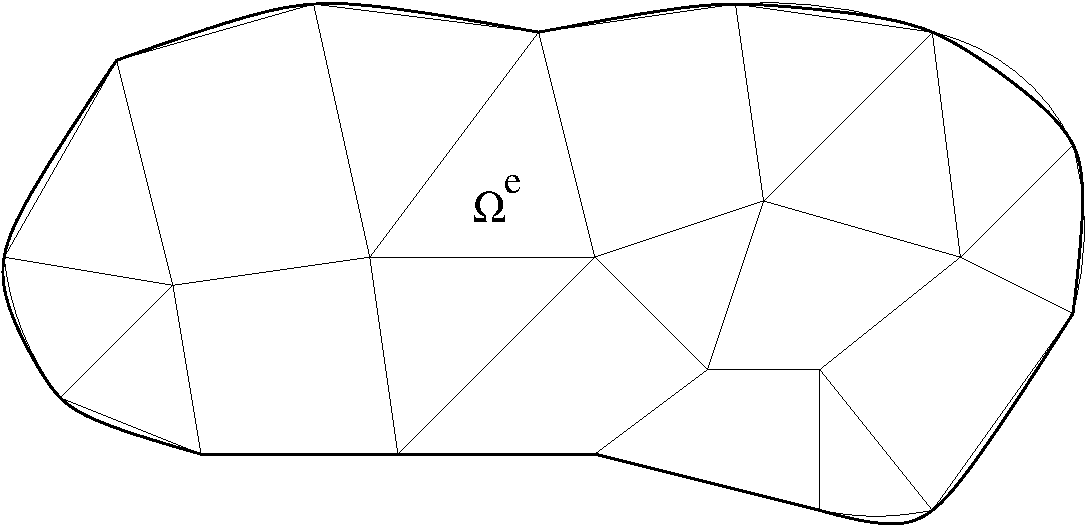
\includegraphics[angle=0,width=0.95\linewidth]
      {finite_element_mesh}
    \end{columns}
  \end{block}
  
  Note that $\normal\times\vF_1=\normal\times\vF_2$ and that
  $ \vF\cdot(\normal \times ( {\bar{\bar{f_r}}}^{-1} \vnabla \times
  \vec{V}) = (\normal\times\vF)\cdot(\normal \times (
  {\bar{\bar{f_r}}}^{-1} \vnabla \times \vec{V} )$

  \framebreak  % %%%%%%%%%%%%%%%%%%%%%%%%%%%%%%%%%%%

   \begin{block}{Between Elements Simulating  a Thin Sheet}
    \begin{columns}
      \column{0.58\textwidth} \centering
       \begin{itemize}\setlength{\itemsep}{0.3\baselineskip}

       \item In general, we need to break continuity on
          
         \begin{itemize}
         \item $\normal\times\vV$ $\Rightarrow$ Duplication of degrees
           of freedom: $\lbrace g\rbrace_1,\lbrace g\rbrace_2$
         \item $\normal\times\vVd$ $\Rightarrow$ The integral
           boundary term can not be omitted
         \end{itemize}

       \item Two linearly independent equations involving four
         magnitudes $\vE_1,\vE_2,\vH_1,\vH_2$:
         \begin{equation*}
          [~]_{2x2}\, \lbrace X \rbrace_{2x1}=\lbrace B \rbrace_{2x1}
        \end{equation*}

      \item \alert{Different possibilities depending on the magnitudes chosen
        as sources (right hand side $B$) and responses $X$}

      \item Clear analogy with two-port network parameters of linear
        circuit analysis: \\
        {\centering$\vE\leftrightarrow V \qquad \vH\leftrightarrow I$}
        % \begin{itemize}
        % \item $\vE\leftrightarrow V$
        % \item $\vH\leftrightarrow I$
        % \end{itemize}
      \end{itemize}
      
      \column{0.4\textwidth} \centering
      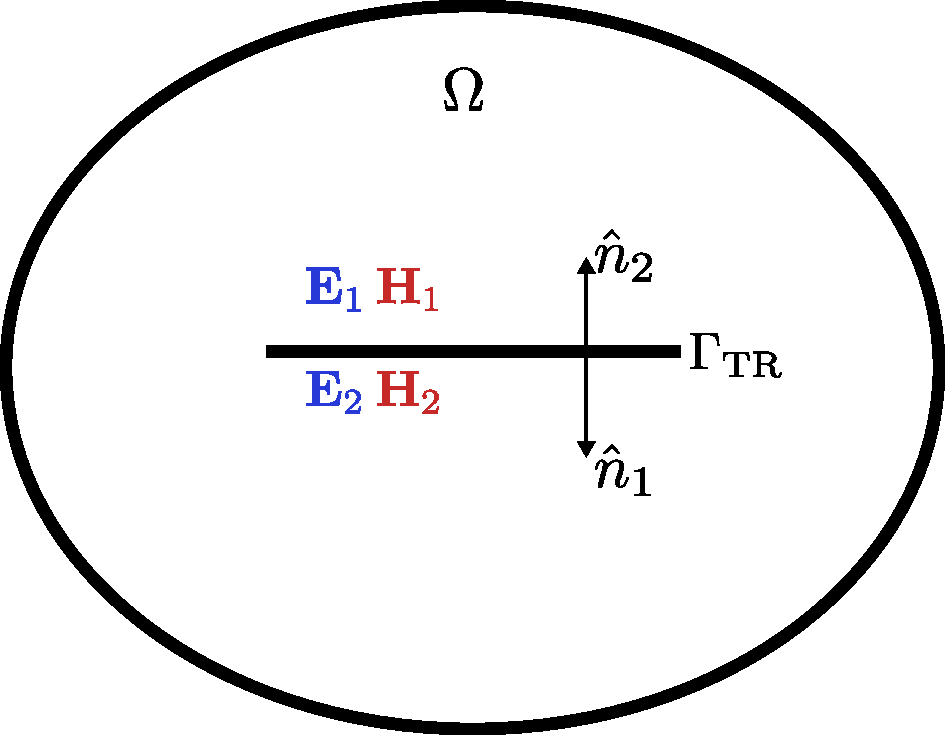
\includegraphics[angle=0,width=\textwidth]{scenario.pdf}
    \end{columns}
   \end{block}

\end{frame}

% %%%%%%%%%%%%%%%%%%%%%%%%%%%%%%%%%%%%%%%%%%%%%%%%%%%%%%%%%%%%%%%%%%%%%%%%%

\begin{frame}[allowframebreaks]{The Immittance Approach}{The Simplest (Least Invasive)
    Approach}
  
  \begin{itemize}\setlength{\itemsep}{0.3\baselineskip}
  \item We express $\normal\times\vVd$ for region~1 and region~2 in terms of 
    $\normal\times\vV$ of region~1 and region~2, i.e.,
    %
    \begin{equation*}
      \begin{Bmatrix}
        \normal\times\vVd_1 \\ \normal\times\vVd_2
      \end{Bmatrix} =
      \begin{bmatrix}
        YZ_{11} & YZ_{12} \\ YZ_{21}  & YZ_{22}
      \end{bmatrix}
      \begin{Bmatrix}
        \normal\times\vV_1 \\ \normal\times\vV_2
      \end{Bmatrix} 
    \end{equation*}

    \begin{itemize}
    \item  This is equivalent to an immitance characterization of
      the equivalent two-port network connecting upper and lower
      regions separated by the sheet.
      % 
      \begin{itemize}
      \item Form.\ $\vE$: $\vV=\vE$, $\vVd=\vH$, immittance $\equiv$ admitance 
      \item Form.\ $\vE$: $\vV=\vE$, $\vVd=\vH$, immittance $\equiv$ impedance 
      \end{itemize}
    \end{itemize}

  \item We substitute $\normal\times\vVd$ on the integral boundary
    terms corresponding to region~1 and region~2 by its linear
    combination of $\normal\times\vV_1$ and $\normal\times\vV_2$.

    \framebreak  % %%%%%%%%%%%%%%%%%%%%%%%%%%%%%%%%%%%
    
  \item For instance, with $\vE$-formulation we have

    \begin{multline*}
      \int_{\Gamma} \vF_1\cdot(\normal \times ( {\bar{\bar{\mu_r}}}^{-1} \vnabla \times \vec{E}_1 )) d\Gamma = \\
      y_{11}\int_{\Gamma} \vF_1\cdot(\normal  \times \vec{E}_1 )) d\Gamma
      + y_{12}\int_{\Gamma} \vF_1\cdot(\normal  \times \vec{E}_2 )) d\Gamma
    \end{multline*}
    \begin{multline*}
      \int_{\Gamma} \vF_2\cdot(\normal \times ( {\bar{\bar{\mu_r}}}^{-1} \vnabla \times \vec{E}_2 )) d\Gamma = \\
      y_{21}\int_{\Gamma} \vF_2\cdot(\normal  \times \vec{E}_1 )) d\Gamma
      + y_{22}\int_{\Gamma} \vF_2\cdot(\normal  \times \vec{E}_2 )) d\Gamma
    \end{multline*}
      % 
    where $\normal\times\vF_1=\normal\times\vF_2$ (conformal mesh
    above-below the sheet).

 
  \item Thus, the TX/RX continuity conditions imposed by the sheet are
    translated into algebra simply as extra contributions for the
    values of the matrix coefficients (related to the duplicated
    degrees of freedom $\lbrace g\rbrace_1$, $\lbrace g\rbrace_2$
    associated to the sheet).

    \begin{block}{Advantages}
      \begin{itemize}
      \item Simple (non code invasing)
        \begin{itemize}
        \item No new variational unknowns
        \item No new equations but simply additional terms to the
          existing ones
        \item Only requires replication of uknonws on sheet:
          $\lbrace g\rbrace_1\ne\lbrace g\rbrace_2$
        \end{itemize}
      \item Reciprocity of the material ($y_{12}=y_{21}$)
        $\Rightarrow$ symmetry of FEM matrix
      \item Short circuit (PEC) and open circuit (PMC) conditions
        naturally reproducible
      \end{itemize}
    \end{block}

    \begin{block}{Disadvantages}
      \begin{itemize}
      \item Total transmission (sheet transparency) \alert{not reproducible}
        \begin{itemize}
        \item \alert{Singular} system of equations
        \item This situation must be either avoided or taken into
          account explicitly
        \end{itemize}
      \end{itemize}
    \end{block}

  \end{itemize}

\end{frame}
  
% %%%%%%%%%%%%%%%%%%%%%%%%%%%%%%%%%%%%%%%%%%%%%%%%%%%%%%%%%%%%%%%%%%%%%%%%%

\begin{frame}[allowframebreaks]{The Immittance Approach}{Special Cases}
  
  \begin{block}{Short Circuit (PEC) Sheet}
    \begin{itemize}
    \item We have $y_{12}=y_{21}=0$ and $y_{11}=y_{22}=\infty$
    \item Thus, the equation associated to $\lbrace g\rbrace_1$ has
      a dominant term 
%      
      \begin{equation*}
        \ldots + y_{11} \int_{\Gamma} \vF_1\cdot(\normal  \times \vec{E}_1 )) d\Gamma
        + y_{12}\int_{\Gamma} \vF_1\cdot(\normal  \times \vec{E}_2 )) d\Gamma
        \approx
        \infty \int_{\Gamma} \vF_1\cdot(\normal  \times \vec{E}_1 )) d\Gamma
      \end{equation*}
    %  
     that corresponds to impose $\normal\times\vec{E}_1=0$,
      i.e., algebraically $\lbrace g\rbrace_1=0$
      
    \item Analogously, with equation associated to
      $\lbrace g\rbrace_2$
      \begin{equation*}
        \ldots + y_{21} \int_{\Gamma} \vF_2\cdot(\normal  \times \vec{E}_1 )) d\Gamma
        + y_{22}\int_{\Gamma} \vF_2\cdot(\normal  \times \vec{E}_2 )) d\Gamma
        \approx
        \infty \int_{\Gamma} \vF_2\cdot(\normal  \times \vec{E}_2 )) d\Gamma
      \end{equation*}
    %  
     that corresponds to impose $\normal\times\vec{E}_2=0$,
      i.e., algebraically $\lbrace g\rbrace_2=0$
      
    \end{itemize}
  \end{block}
  
  \framebreak  % %%%%%%%%%%%%%%%%%%%%%%%%%%%%%%%%%%%
  
  \begin{block}{Open Circuit (PMC) Sheet}
    \begin{itemize}
    \item We have $y_{12}=y_{21}=0$ and $y_{11}=y_{22}=0$
    \item Thus, the equation associated to $\lbrace g\rbrace_1$ is
      equivalent to have
%      
      \begin{equation*}
        \int_{\Gamma} \vF_1\cdot(\normal \times ( {\bar{\bar{\mu_r}}}^{-1} \vnabla \times \vec{E}_1 )) d\Gamma = 0
      \end{equation*}
    %  
      that corresponds to weakly impose
      $\normal\times{\bar{\bar{\mu_r}}}^{-1}\vnabla\times\vec{E}_1=0$ (Neumann b.c.)  i.e.,
      $\normal\times\vec{H}_1=0$.
      
    \item Analogously, with equation associated to
      $\lbrace g\rbrace_2$
      \begin{equation*}
        \int_{\Gamma} \vF_2\cdot(\normal \times ( {\bar{\bar{\mu_r}}}^{-1} \vnabla \times \vec{E}_2 )) d\Gamma = 0
      \end{equation*}
    %  
      that corresponds to weakly impose
      $\normal\times{\bar{\bar{\mu_r}}}^{-1}\vnabla\times\vec{E}_2=0$ (Neumann b.c.)  i.e.,
      $\normal\times\vec{H}_2=0$.
    \end{itemize}
  \end{block}
  
  \framebreak  % %%%%%%%%%%%%%%%%%%%%%%%%%%%%%%%%%%%
  
  \begin{block}{Total Transmission (sheet transparency)}
    \begin{itemize}
    \item It is clear that from
      % 
      \begin{equation*}
        \begin{Bmatrix}
          \normal\times\vVd_1 \\ \normal\times\vVd_2
        \end{Bmatrix} =
        \begin{bmatrix}
          YZ_{11} & YZ_{12} \\ YZ_{21}  & YZ_{22}
        \end{bmatrix}
        \begin{Bmatrix}
          \normal\times\vV_1 \\ \normal\times\vV_2
        \end{Bmatrix} 
      \end{equation*}
      % 
      is not possible to impose full continuity of $\normal\times\vV$,
      $\normal\times\vVd$, i.e., 
      % 
      \begin{equation*}
        \begin{Bmatrix}
          \normal\times\vV_1 \\ \normal\times\vVd_1
        \end{Bmatrix} =
        \begin{Bmatrix}
          \normal\times\vV_2 \\ \normal\times\vVd_2
        \end{Bmatrix} 
      \end{equation*}
      
    \item Technically, we have $y_{12}=y_{21}=\infty$ and $y_{11}=y_{22}=\infty$
      
    \end{itemize}
  \end{block}
  
  \framebreak  % %%%%%%%%%%%%%%%%%%%%%%%%%%%%%%%%%%%

  \begin{block}{Total Transmission (sheet transparency)}
    \begin{itemize}
    
  \item Thus, the equation associated to $\lbrace g\rbrace_1$ has
      two dominant terms 
%      
      \begin{equation*}
        \ldots + \infty \int_{\Gamma} \vF_1\cdot(\normal  \times \vec{E}_1 )) d\Gamma
        + \infty \int_{\Gamma} \vF_1\cdot(\normal  \times \vec{E}_2 )) d\Gamma
      \end{equation*}
      
    \item Analogously, with equation associated to
      $\lbrace g\rbrace_2$
      \begin{equation*}
        \ldots + \infty \int_{\Gamma} \vF_2\cdot(\normal  \times \vec{E}_1 )) d\Gamma
        + \infty \int_{\Gamma} \vF_2\cdot(\normal  \times \vec{E}_2 )) d\Gamma
      \end{equation*}
      
    \end{itemize}
  \end{block}

  \begin{alertblock}{Total Transmission (sheet transparency)}%{Singular System of Equations}
    \begin{itemize}
    \item Both equations tends to be the same equation
      \begin{itemize}
      \item[$\Rightarrow$] Singular FEM matrix
      \end{itemize}
      \alert{(I mush still check signs for $y_{ij}$) } Nevertheless,
      the above resulting equations can never impose continuity of
      $\normal\times\vV$
    \end{itemize}
  \end{alertblock}
  
  \framebreak  % %%%%%%%%%%%%%%%%%%%%%%%%%%%%%%%%%%%

  \begin{block}{%Total Transmission (sheet transparency)
      Workaround}
    \begin{itemize}
    \item We must identify the case, i.e., when $y_{ij}$ is
      \alert{``large enough''}
      
    \item Then, we have two main possibilities:
      \begin{itemize}
      \item \alert{Ignore}  TR/RX boundary conditions for that sheet, i.e., do nothing  
        \begin{itemize}
        \item Do not replicate  degres of freedom $\lbrace g\rbrace$
        \item Do not alter FEM equations
        \end{itemize}
      \item \alert{Recover} full continuity, i.e., continuity of
        $\normal\times\vV$ and $\normal\times\vVd$ once replication of
        $\lbrace g\rbrace$ has been perfomed
        \begin{itemize}
        \item Several possibilities
        \end{itemize}
      \end{itemize}

    \end{itemize}
  \end{block}
      
  \framebreak  % %%%%%%%%%%%%%%%%%%%%%%%%%%%%%%%%%%%

  \begin{center}
    How to Recover Full Continuity?
  \end{center}

  \begin{itemize}
  \item We keep  the integral boundary term $\int_{\Gamma} \vF\cdot(\normal \times ( {\bar{\bar{f_r}}}^{-1} \vnabla \times \vec{V} )) d\Gamma$
    for region~1 and region~2

  \item We add two equations to recover continuity of
    $\normal\times\vV$ and $\normal\times\vVd$
    \end{itemize}
    
  \begin{block}{Continuity of  $\normal\times\vV$}
    \begin{itemize}
    \item We add one strong condition equation
      %
      \begin{equation*}
         \lbrace g\rbrace_1 =  \lbrace g\rbrace_2 
      \end{equation*}

    \item Perfomed at the algebraic level, 
      % (similar to the setting of  Dirichlet boundary conditions),
      i.e., operating in the matrix by fixing all coefficients on the
      corresponding row to zero except the two being related (paired)

    \item The above operation is simple, trivial I would say.

    \item However,  it introduces asymmetry
      in the FEM matrix
      
    \end{itemize}
  \end{block}
  
  \framebreak  % %%%%%%%%%%%%%%%%%%%%%%%%%%%%%%%%%%%

  \begin{block}{Continuity of $\normal\times\vVd$, i.e., of
      $\normal\times( {\bar{\bar{f_r}}}^{-1} \vnabla \times\vV)$}
    \begin{itemize}
    \item We add a equation to weakly force continuity of the dual variable
      %
      \begin{equation}
        \label{eq:weakrecoverVd}
        \int_{\Gamma} \vF_1\cdot(\normal \times ( {\bar{\bar{\mu_r}}}^{-1} \vnabla \times \vec{E}_1 )) d\Gamma = 
        \int_{\Gamma} \vF_2\cdot(\normal \times ( {\bar{\bar{\mu_r}}}^{-1} \vnabla \times \vec{E}_2 )) d\Gamma 
      \end{equation}

    \item Note that the above equation after discretization introduces
      asymmetry in the matrix
      \begin{itemize}
      \item Although, $\normal\times\vF_1=\normal\times\vF_2$ due to
        conformity of the mesh
      \item the discretization of
        $\normal \times \vnabla\times\vec{E}$ involves all basis
        functions of the finite element, i.e., not only basis
        functions on the common boundary (sheet)
      \end{itemize}

      
    \end{itemize}
  \end{block}

  \framebreak  % %%%%%%%%%%%%%%%%%%%%%%%%%%%%%%%%%%%

  \begin{center}
    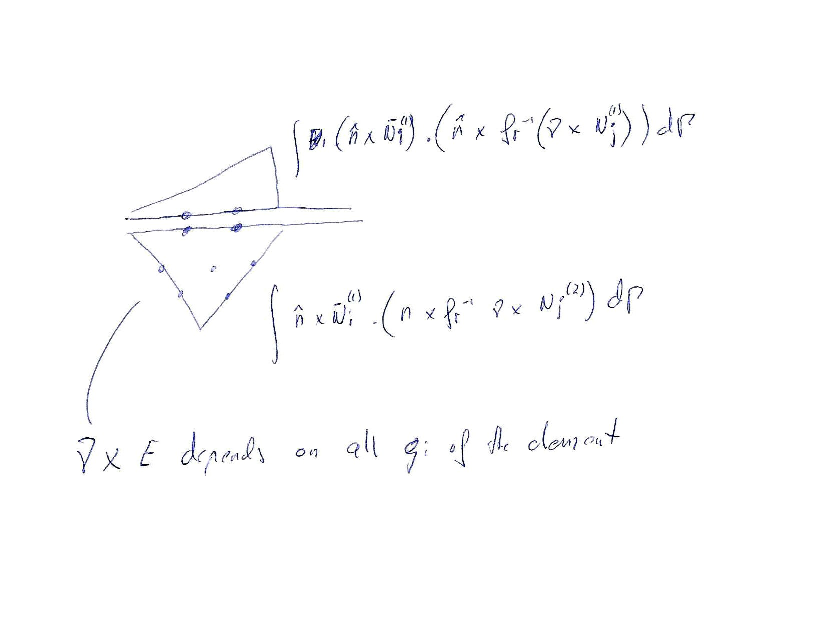
\includegraphics[angle=0,width=0.6\textwidth]{ilustracion_weakrecoverVd}
  \end{center}
  
  \framebreak  % %%%%%%%%%%%%%%%%%%%%%%%%%%%%%%%%%%%
  
  \begin{itemize}
  \item The above procedure of recovering full continuity can also be
    approached by defining a new variational unknown for the dual
    field, i.e., for $\normal\times\vVd$; basically,
    \begin{itemize}
    \item A $\vJ$ for $\vE$-formulation
    \item A $\vM$ for $\vH$-formulation
    \end{itemize}
    
  \item Once being involved with new variational uknowns it is much
    worthier to consider other approaces (\alert{described later in
      this presentation??})
    
  \end{itemize}
      
  \framebreak  % %%%%%%%%%%%%%%%%%%%%%%%%%%%%%%%%%%%

  \begin{center}
    How to Recover Full Continuity? (EQUIVALENT METHOD) \\ \alert{need
      to think twice if is really equivalent}
  \end{center}

  \begin{itemize}
  \item We use ABCs in each region, i.e., we substitute in the integral
    boundary term of region~1 and region~2 as follows
    $\int_{\Gamma} \vF\cdot(\normal \times ( {\bar{\bar{f_r}}}^{-1}
    \vnabla \times \vec{V} )) d\Gamma$ with

    \begin{equation*}
      \begin{split}
        \int_{\Gamma} \vF_1\cdot(\normal \times ( {\bar{\bar{f_r}}}^{-1} \vnabla \times \vec{V}_1 )) \,d\Gamma
        &= 
        jk_0 \int_{\Gamma} \left( \normal \times \vec{F}_1 \right) \cdot \left( \normal \times \vec{V}_1 \right) d\Gamma_\text{C}
        \\
        \int_{\Gamma} \vF_2\cdot(\normal \times ( {\bar{\bar{f_r}}}^{-1} \vnabla \times \vec{V}_2 )) \,d\Gamma
        &= 
        jk_0 \int_{\Gamma} \left( \normal \times \vec{F}_2 \right) \cdot \left( \normal \times \vec{V}_2 \right) d\Gamma_\text{C}
      \end{split}
    \end{equation*}

    This is trivial

    \item We add one strong condition equation
      %
      \begin{equation*}
         \lbrace g\rbrace_1 =  \lbrace g\rbrace_2 
      \end{equation*}
    \end{itemize}
      
  \end{frame}

% %%%%%%%%%%%%%%%%%%%%%%%%%%%%%%%%%%%%%%%%%%%%%%%%%%%%%%%%%%%%%%%%%%%%%%%%%

\begin{frame}[allowframebreaks]{The $[g]$, $[h]$, $[ABCD]$ Approaches}
  
  \begin{columns}[T]
    \column{0.45\textwidth} \centering
    \begin{block}{$[g]$ Parameters}
      \begin{equation*}
        \begin{Bmatrix}  I_1 \\ V_2 \end{Bmatrix} =
        \begin{bmatrix}    g_{11} & g_{12} \\ g_{21}  & g_{22}  \end{bmatrix}
        \begin{Bmatrix}  V_1 \\ I_2  \end{Bmatrix} 
      \end{equation*}
    \end{block}
    
    \column{0.45\textwidth} \centering
    \begin{block}{$[h]$ Parameters}
      \begin{equation*}
        \begin{Bmatrix}  V_1 \\ I_2  \end{Bmatrix} =
        \begin{bmatrix}    h_{11} & h_{12} \\ h_{21}  & h_{22}  \end{bmatrix}
        \begin{Bmatrix}  I_1 \\ V_2 \end{Bmatrix} 
      \end{equation*}
    \end{block}
    
    \end{columns}

    \vbs
    
    \begin{columns}
    \column{0.45\textwidth} \centering
    \begin{block}{$[ABCD]$ Parameters}
      \begin{equation*}
        \begin{Bmatrix}  V_1 \\ I_1  \end{Bmatrix} =
        \begin{bmatrix}   A & B \\ C & D  \end{bmatrix}
        \begin{Bmatrix}  V_2 \\ I_2 \end{Bmatrix} 
      \end{equation*}
    \end{block}
  \end{columns}

%  \framebreak  % %%%%%%%%%%%%%%%%%%%%%%%%%%%%%%%%%%%


%    \begin{block}{Ideal Transformer}
% %     \begin{columns}
% %       \column{0.45\textwidth} \centering
%        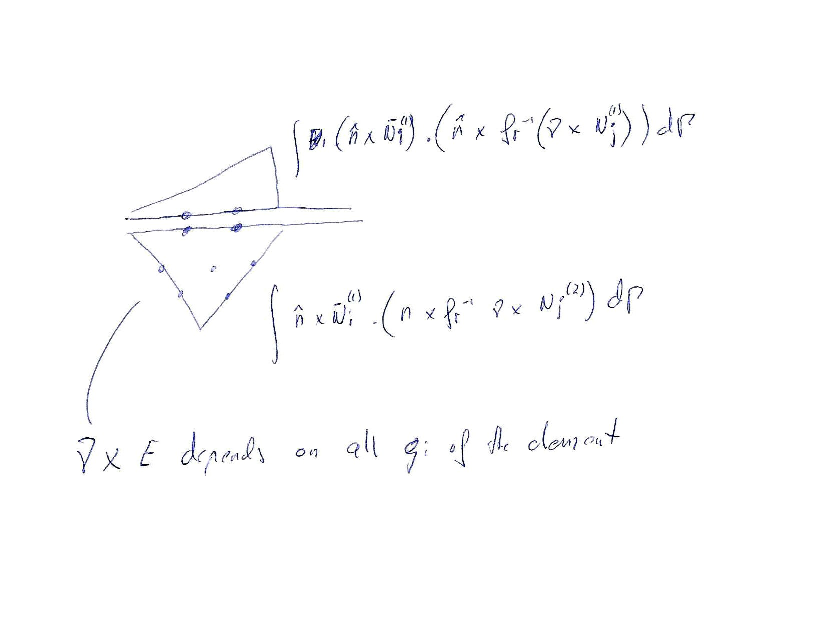
\includegraphics[angle=0,width=0.8\textwidth]{ilustracion_weakrecoverVd}
% %       \column{0.45\textwidth} \centering
 % \begin{equation*}
 %   \begin{bmatrix}   A & B \\ C & D  \end{bmatrix}
 %    = 
 %   \begin{bmatrix}   \frac{1}{n} & 0 \\ 0 & n  \end{bmatrix}
 % \end{equation*}
 % \begin{equation*}
 %   \begin{bmatrix}    h_{11} & h_{12} \\ h_{21}  & h_{22}  \end{bmatrix}
 %    = 
 %   \begin{bmatrix}   0 & \frac{1}{n} \\ -\frac{1}{n} & 0  \end{bmatrix}
 % \end{equation*}
% %   \end{columns}
      
%    \end{block}

      
\end{frame}

% %%%%%%%%%%%%%%%%%%%%%%%%%%%%%%%%%%%%%%%%%%%%%%%%%%%%%%%%%%%%%%%%%%%%%%%%%

\begin{frame}[allowframebreaks]{The $[g]$, $[h]$, $[ABCD]$
    Approaches}{Total Transmission (sheet transparency)}
  
  \begin{block}{Analogy: Ideal Transformer}
     \begin{columns}
       \column{0.45\textwidth} \centering
    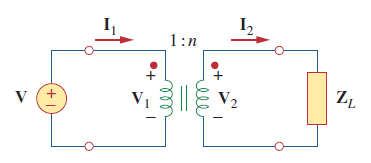
\includegraphics[angle=0,width=\textwidth]{ideal_transformer}
     \column{0.45\textwidth} \centering
    \begin{equation*}
      \begin{bmatrix}   A & B \\ C & D  \end{bmatrix}
      = 
      \begin{bmatrix}   \frac{1}{n} & 0 \\ 0 & n  \end{bmatrix}
    \end{equation*}
    \begin{equation*}
      \begin{bmatrix}    h_{11} & h_{12} \\ h_{21}  & h_{22}  \end{bmatrix}
      = 
      \begin{bmatrix}   0 & \frac{1}{n} \\ -\frac{1}{n} & 0  \end{bmatrix}
    \end{equation*}
    \end{columns}
    
  \end{block}


\end{frame}

% %%%%%%%%%%%%%%%%%%%%%%%%%%%%%%%%%%%%%%%%%%%%%%%%%%%%%%%%%%%%%%%%%%%%%%%%%

\begin{frame}[allowframebreaks]{The $[g]$, $[h]$, $[ABCD]$
    Approaches}{FEM Implementation}

  \begin{itemize}
  \item Duplication of degrees of freedom:
    $\lbrace g\rbrace_1,\lbrace g\rbrace_2$
  \item Keeping the integral boundary terms in region~1 and region~2

  \item Adding two equations to weakly enforce the corresponding
    tranmsision conditions (given by $[g]$, $[h]$, $[ABCD]$, etc)
    
    \begin{itemize}
    \item  Optionally, definition of a new variational unknown
      for the dual field, i.e., for $\normal\times\vVd$; basically,
    \begin{itemize}
    \item A $\vJ$ for $\vE$-formulation
    \item A $\vM$ for $\vH$-formulation
    \end{itemize}
    for helping to set the equations
  \end{itemize}

    
    
  \end{itemize}

  
\end{frame}

% %%%%%%%%%%%%%%%%%%%%%%%%%%%%%%%%%%%%%%%%%%%%%%%%%%%%%%%%%%%%%%%%%%%%%%%%%

  \begin{frame}[plain]
    \centering \Large{Elaborar sobre la muy buena idea de Sergio de ¡utilizar
      relaciones lineales entre combinaciones de V e I como sucede en
      la caraterización con los parámetros S}
    
  \end{frame}



% %%%%%%%%%%%%%%%%%%%%%%%%%%%%%%%%%%%%%%%%%%%%%%%%%%%%%%%%%%%%%%%%%%%%%%%%%
\subsection{Two-Port Network Parameters}
% %%%%%%%%%%%%%%%%%%%%%%%%%%%%%%%%%%%%%%%%%%%%%%%%%%%%%%%%%%%%%%%%%%%%%%%%%

\begin{frame}{TITULO}
  Hola
\end{frame}




% %%%%%%%%%%%%%%%%%%%%%%%%%%%%%%%%%%%%%%%%%%%%%%%%%%%%%%%%%%%%%%%

\section{$[Z]$/$[Y]$ Approach}

  \begin{frame}[plain]
    \centering \Large{We describe the implementation of the TX/RX
      conditions uisng the characterization of the material sheet in terms of
      its immittance (impedance/admittance) matrix}
    
  \end{frame}

  %%%%%%%%%%%%%%%%%%%%%%%%%%%%%%%%%%%%%%%%%%%%%%%%%%%%%%%%%%%%%%%%%%%%%%%%% 
% $Id$
% %%%%%%%%%%%%%%%%%%%%%%%%%%%%%%%%%%%%%%%%%%%%%%%%%%%%%%%%%%%%%%%%%%%%%%%%%
%
% Set de slides estudiando diferencias entre uso de Green3D o Green2D
% para problema cilindro infinito usando una seccion (rodaja 3D) del
% cilindro
%
% %%%%%%%%%%%%%%%%%%%%%%%%%%%%%%%%%%%%%%%%%%%%%%%%%%%%%%%%%%%%%%%%%%%%%%%%%

% %%%%%%%%%%%%%%%%%%%%%%%%%%%%%%%%%%%%%%%%%%%%%%%%%%%%%%%%%%%%%%%%%%%%%%%%%
\subsection{FEM Formulation}
% %%%%%%%%%%%%%%%%%%%%%%%%%%%%%%%%%%%%%%%%%%%%%%%%%%%%%%%%%%%%%%%%%%%%%%%%%

\begin{frame}[allowframebreaks]{Formulation}
  \begin{columns}
    \column{0.4\textwidth} \centering
    {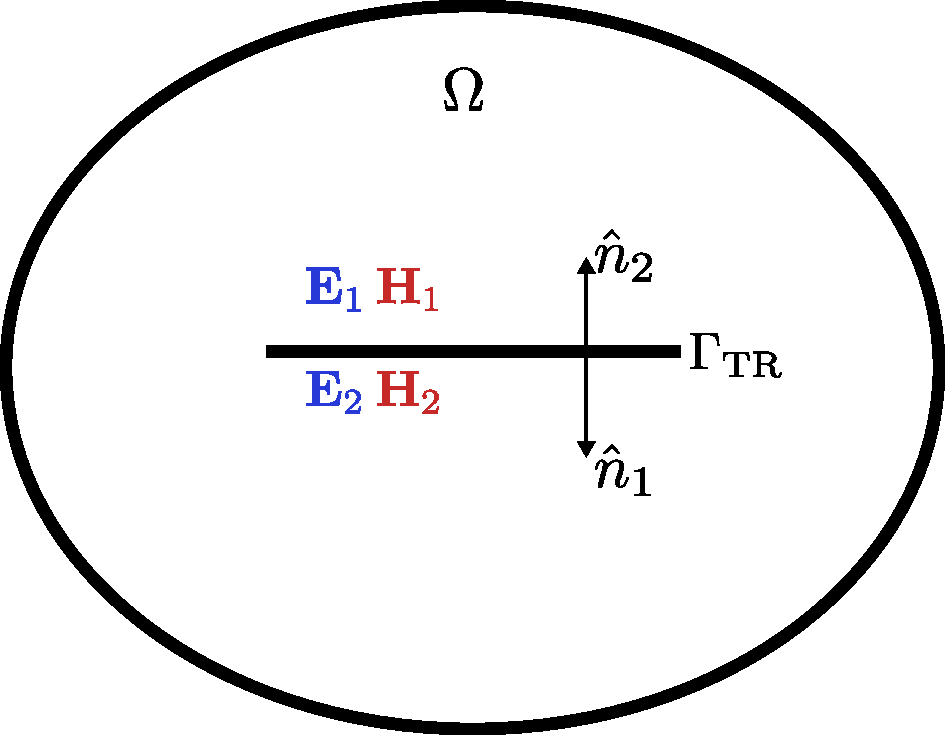
\includegraphics[angle=0,width=\textwidth]{scenario.pdf}}
    \column{0.6\textwidth}
    {
      \begin{align*}
        \hat{n}_1\times(\mu_r^{-1}&\nabla\times\vec{E}_1) - \frac{jk_0}{\eta}y_{11}\hat{n}_1\times(\hat{n}_1\times\vec{E}_1) - \\
        - &\frac{jk_0}{\eta}y_{12}\hat{n}_2\times(\hat{n}_2\times\vec{E}_2) = 0,
      \end{align*}
      \begin{align*}
        \hat{n}_2\times(\mu_r^{-1}&\nabla\times\vec{E}_2) - \frac{jk_0}{\eta}y_{21}\hat{n}_1\times(\hat{n}_1\times\vec{E}_1) - \\
        - &\frac{jk_0}{\eta}y_{22}\hat{n}_2\times(\hat{n}_2\times\vec{E}_2) = 0,
      \end{align*}

      \alert{Note that $y_{\rm xx}$ are relative to the vacuum admittance.}
    }
  \end{columns}

  \framebreak % %%%%%%%%%%%%%%%%%%%%%%%%%%%%%%%%%%%%%%

  Find $\vec{E} \in \vec{H}_0(\text{curl},\Omega)$ such that
  \begin{align*}
    &\Big(\nabla\times\vec{w},\mu_r^{-1}\nabla\times\vec{E} \Big)_\Omega - k_0^2\Big(\vec{w},\varepsilon_r\vec{E} \Big)_\Omega + 
    jk_0\Big\langle\hat{n}\times\vec{w},\hat{n}\times\vec{w}\Big\rangle_{\Gamma_{\text{C}}} = \\
    &\;\Big(\vec{w},\vec{F}\Big)_\Omega - 
    \Big\langle\hat{n}\times(\vec{w}\times\hat{n}),\vec{\Psi}_{\text{N}}\Big\rangle_{\Gamma_{\text{N}}} -
    \Big\langle\hat{n}\times(\vec{w}\times\hat{n}),\vec{\Psi}_{\text{C}}\Big\rangle_{\Gamma_{\text{C}}}
    \quad \forall \,\vec{w} \in \vec{H}_0(\text{curl},\Omega).
  \end{align*}
  
  with
  \begin{align}
    \Big(\vec{w},\vec{v}\Big)_\Omega &= \int_\Omega \vec{w}^* \cdot \vec{v} d\Omega, \nonumber\\
    \Big\langle \vec{w},\vec{v}\Big\rangle_{\Gamma} &= \int_\Gamma \vec{w}^* \cdot \vec{v} d\Gamma.\nonumber
  \end{align}
  
  \framebreak % %%%%%%%%%%%%%%%%%%%%%%%%%%%%%%%%%%%%%%
  For \emph{upper} elements on $\Gamma_{\rm TR}$ (side 1), we have
  \small
  \begin{align*}
    &{\rm LHS_1} \\
    &\; + j\frac{k_0}{\eta}\Big\langle\hat{n}\times(\vec{w}_1\times\hat{n}),y_{11}\hat{n}\times(\vec{w}_1\times\hat{n})\Big\rangle_{\Gamma_{\text{TR}}} + j\frac{k_0}{\eta}\Big\langle\hat{n}\times(\vec{w}_1\times\hat{n}),y_{12}\hat{n}\times(\vec{w}_2\times\hat{n})\Big\rangle_{\Gamma_{\text{TR}}} = \\
    &\;\;{\rm RHS_1},
  \end{align*}
  \normalfont
  whereas for \emph{lower} elements (side 2), we get
  \small
  \begin{align*}
    &{\rm LHS_2} \\
    &\; + j\frac{k_0}{\eta}\Big\langle\hat{n}\times(\vec{w}_2\times\hat{n}),y_{21}\hat{n}\times(\vec{w}_1\times\hat{n})\Big\rangle_{\Gamma_{\text{TR}}} + j\frac{k_0}{\eta}\Big\langle\hat{n}\times(\vec{w}_2\times\hat{n}),y_{22}\hat{n}\times(\vec{w}_2\times\hat{n})\Big\rangle_{\Gamma_{\text{TR}}} = \\
    &\;\;{\rm RHS_2},
  \end{align*}
  \normalfont
\end{frame}

\begin{frame}{FEM implementation}
  \begin{itemize}
    \item The DOFs will be doubled for the faces and the interior edges.
    \item The exterior edges of $\Gamma_{\rm TR}$ are not doubled.
    \begin{itemize}
      \item Identified by code: the edges associated to two faces are interior. 
      \item If the boundaries of the sheet belong to PBC, the edges of $\Gamma_{\rm TR}$ are also doubled.
    \end{itemize}
  \end{itemize}
\end{frame}

% %%%%%%%%%%%%%%%%%%%%%%%%%%%%%%%%%%%%%%%%%%%%%%%%%%%%%%%%%%%%%%%%%%%%%%%%%
\subsection{Testing}
% %%%%%%%%%%%%%%%%%%%%%%%%%%%%%%%%%%%%%%%%%%%%%%%%%%%%%%%%%%%%%%%%%%%%%%%%%

\begin{frame}{Problem to be solved}
  \begin{columns}
    \column{0.48\textwidth} \centering
    {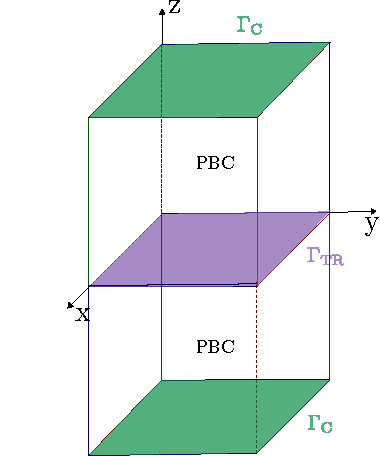
\includegraphics[angle=0,width=\textwidth]{tr_problem.pdf}}
    \column{0.48\textwidth}
    {
      Simulation of an infinite medium with transmission/reflection sheet that divides the space into two halves.
      \begin{itemize}
        \item $\Gamma_\text{TR}$: Transmission/reflection sheet defined with 
        \begin{equation*}
          \vec{Y} = \begin{bmatrix}
            y_{11} & y_{12} \\
            y_{21} & y_{22}
          \end{bmatrix}.
        \end{equation*}
        \item $\Gamma_\text{C}$: ABC with excitation with polarization $E_y$
        \item The vertical faces are set to PBC
      \end{itemize} 
    }
  \end{columns}
\end{frame}

\begin{frame}{Testbench}
  \begin{itemize} 
    \item $\vec{Y} = \begin{bmatrix}
      0 & 0 \\
      0 & 0
    \end{bmatrix}$: sanity check, we should get same result as the two halves with a PMC.
    \item $\vec{Y} = \mathbb{I}$: sanity check, we should get same result as the two halves with an ABC.
    \item Change lower $\Gamma_\text{C}$ by PEC and solve analytic problem with four media: final test.
    \begin{itemize}
      \item Obtain parameters for $\vec{Y}$ of the equivalent problem.
      \item Get same solutions for the electric field.
      \item Transparent? Puede ser que aproximar con $1e6$. Quizás con ABCD.
    \end{itemize}
  \end{itemize}
\end{frame}

% %%%%%%%%%%%%%%%%%%%%%%%%%%%%%%%%%%%%%%%%%%%%%%%%%%%%%%%%%%%%%%%%%%%%%%%%%
\subsection{HOFEM Implementation}
% %%%%%%%%%%%%%%%%%%%%%%%%%%%%%%%%%%%%%%%%%%%%%%%%%%%%%%%%%%%%%%%%%%%%%%%%%

\begin{frame}{HOFEM implementation}
  \begin{itemize}
    \item New boundary condition: \texttt{TRBC}.
    \begin{itemize}
      \item We define a normal, $\hat{n}_{\rm TRBC}$ to detect lower and upper side. Upper side is the closer to $\hat{n}_{\rm TRBC}$.
      \item Definition of $y_{11}$, $y_{12}$, $y_{21}$, and $y_{22}$ as relative values with respect to vacuum admittance.
    \end{itemize}
    \item Two options for implementation 
    \begin{itemize}
      \item Integers defined in \texttt{tetrahedra\_element}.
      \item Allocatable array of $1\times N_{\rm elem, TR}$ where the two positions (stored in boundary conditions module, 
      accessible from \texttt{mesh\_reordering\_module} and \texttt{elementary\_terms\_3D}):
      \begin{enumerate}
        \item $10\times$ Neighbor element identifier (to couple $\vec{w}_2$ and $\vec{w}_1$).
        \item Integer 1,2 (side) (to extract the values of $y_{11}$,$y_{12}$,$y_{21}$, and $y_{22}$).
        % \item Integer 10\texttt{bc\_id}+[1,2] (side) (to extract the values of $y_{11}$,$y_{12}$,$y_{21}$, and $y_{22}$).
      \end{enumerate}
      % the neighbor for elements belonging to $\hat{n}_{\rm TRBC}$ and an integer 10\texttt{bc\_id}+[1,2] (side), located in \texttt{mesh\_object\_module}, accessible from \texttt{mesh\_reordering\_module} and \texttt{elementary\_terms\_3D}.
    \end{itemize}
    \item Significant methods involved:
    \begin{itemize}
      \item Postprocessing over \texttt{reordering\_DOF\_algorithm\_3D}. 
      \item \texttt{calc\_boundary\_3D\_nxNi\_nxNi\_term\_of\_this\_element}.
      \item Construction of the MUMPS-related matrix: different number of
      non-zeros per element, assembly of coupled elements (now single-element
      assembly).
    \end{itemize}   
  \end{itemize}
\end{frame}
%%%%%%%%%%%%%%%%%%%%%%%%%%%%%%%%%%%%%%%%%%%%%%%%%%%%%%%%%%%%%%%%


% %%%%%%%%%%%%%%%%%%%%%%%%%%%%%%%%%%%%%%%%%%%%%%%%%%%%%%%%%%%%%%%%%%%%%%%%%


\end{document}
